\section{Introduction}\label{intro}\sloppy
Since most relational database management systems support only dyadic join operators (joining two tables), an algorithm to choose the ``best'' sequence of two-way joins to achieve a k-way join is a core primitive in almost every query optimizer.
Exhaustive enumeration of all possible join orders is prohibitive for large queries.
Due to new visualization and business intelligence tools that automatically generate queries, the prevalence of increasingly large join queries has sparked a renewed interest to effectively scale up join ordering algorithms~\cite{neumann2018adaptive}. 

In practice, query optimizers leverage a combination of pruning heuristics and/or optimization heuristics to make the search for a good plan efficient.
For example, the classical Selinger optimizer restricts its search to left-deep orders~\cite{selinger1979access}.
Left-deep orders still allow for effective index utilization as the intermediate results can be streamed through each index lookup. 
This heuristic is not universally effective, and, in some database architectures, exactly the opposite heuristic is required (i.e., right-deep plans)~\cite{gerber1986data}.
Similarly, there are countless other techniques that exploit other special problem settings, intelligently combine heuristics, or approximate the cost function~\cite{swami1993polynomial,steinbrunn1997heuristic,galindo2008optimizing,ziane1993parallel}. 
For some of methods, precise conditions for optimality are known~(e.g., IK-KBZ~\cite{krishnamurthy1986optimization}). However, for others, given a particular cost function, database, and query workload, it can be very unclear whether the heuristic applies. 

This is not simply an academic concern, and it can be experimentally shown on existing join optimization benchmarks.
Figure \ref{teaser} illustrates this point on a query from the Join Order Benchmark~\cite{leis2015good}, which bases its dataset and queries from the International Movie Database (IMDB). We implemented two different cost models, one similar to~\cite{leis2015good} with a hash-join cost that is linear in the size of the input relations, and one that is similar to the cost models discussed in~\cite{ziane1993parallel} that allows for reuse of already built hash tables.
We use a left-deep dynamic program and a right-deep dynamic program to optimize the joins in the query.
In the first cost model, the best left-deep plan has a 39x lower cost than the best right-deep plan. While in the second cost model, the best right-deep plan has an 8x lower cost than the best left-deep one.
This illustrates that practically, the search problem is unforgiving, where a poor heuristic may suffer orders of magnitudes of optimality.

\begin{figure}
    \centering
    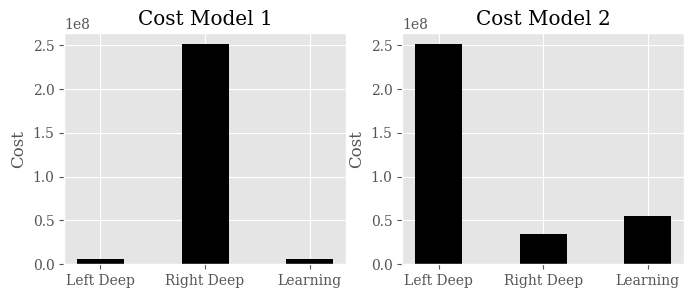
\includegraphics[width=\columnwidth]{figs/teaser.png}
    \caption{\small Query 12b from the Join Order Benchmark with 2 different cost models. Cost model 1 models a hash-join operator with a linear cost in the size of the input relations, and Cost model 2 models re-use of already built hash tables. A learning-based strategy is competitive with the dominant heuristic in both models. \label{teaser}}
\end{figure}

In these dynamic programs, the optimizer incrementally builds optimal joins on subsets of relations.
Leveraging the principle of optimality, it memoizes the optimal join order up-to the current intermediate results.
For a static database, suppose one could hypothetically store all the memoization tables created for all planning instances.
If we had this hypothetical scenario, as the optimizer plans for more queries there is increasing re-use as all possible subplans are covered.
Once this table is fully populated, join ordering would reduce to a hash-table lookup.
In practice, this table would be impossible to fully populate and store.

What if one could represent all of that information with a parametrized statistical model? To do so, we can take inspiration from the Artificial Intelligence field of reinforcement learning (RL)~\cite{sutton1998reinforcement}. RL algorithms use sampling and statistical machine learning to efficiently estimate the long-term benefit of certain decisions.
In our context, this means approximate the query optimizer's cost-to-go function, or what is the long-term value of making a particular join. 
Since the cost-to-go function can be very complex, we sufficiently rich class of functions, like neural networks, to model it.
This is exactly an instance of a Deep RL  algorithm, called Deep Q Networks (DQN), similar to the ones used to play Atari Games or the game of Go.
Going back to Figure \ref{teaser}, we train an RL model on 80 randomly selected queries from the Join Order benchmark and use the learned model to optimize the same query. We find that it is competitive on both cost models.

While the efficacy of machine learning in database internals is still the subject of significant debate~\cite{btree, kraska2018case, mitzenmacher2018model}, we believe that learning strategies for join ordering is a natural fit due to the orders of magnitude of performance at stake. 
This learning based approach gives us flexibility in designing new intelligent enumeration strategies by manipulating how the neural network is trained and how it represents the subplans.
For example, the neural network allows us to efficiently share query processing information across planning instances with the neural network parameters and learn from previously executed queries.
The consequence is enumeration strategies tuned to the specific workload and data.
We can also vary the features used to represent the subplans, to allow the network to capture different properties physical operator selection and selectivities.
We can also train the neural network with observations of actual query execution times and make it robust to faulty cost models.

In short, Deep RL provides a new algorithmic perspective for thinking about join enumeration. 
The essence is to shift the cost of heuristic design to data collection and featurization.
Our system, called \sys, is built on Apache Calcite and we present extensive results on the join order benchmark.
We show \sys optimizes plans well across many different cost models for a relatively modest set of training queries.
Admittedly, this raises a new set of problems including overfitting and avoiding high-variance plans.
We hope that \sys is a first step in an entire spectrum of techniques between pure Deep RL and classical query optimization.


 

